\documentclass[journal]{IEEEtran}

\usepackage{ifpdf}
 \ifpdf
   % pdf code
 \else
   % dvi code
 \fi
\usepackage{cite}
\ifCLASSINFOpdf
  \usepackage[pdftex]{graphicx}
   %\graphicspath{{../pdf/}{../jpeg/}}
   \DeclareGraphicsExtensions{.pdf,.jpeg,.png}
\else
  \usepackage[dvips]{graphicx}
  %\graphicspath{{../eps/}}
  \DeclareGraphicsExtensions{.eps}
\fi
\usepackage[cmex10]{amsmath}
\usepackage{algorithmic}
\usepackage{array}
\usepackage{mdwmath}
\usepackage{mdwtab}
\usepackage{eqparbox}
\usepackage[caption=false,font=footnotesize]{subfig}
\usepackage{fixltx2e}
\usepackage{url}
\usepackage{color}

\newenvironment{meta}[0]{\color{red} \em}{}

% correct bad hyphenation here
\hyphenation{op-tical net-works semi-conduc-tor}


\begin{document}

\title{The Rao-Blackwellised \\ Variable Rate Particle Smoother for \\ Conditionally Linear-Gaussian Models}

\author{Pete~Bunch,~\IEEEmembership{}
        Simon~Godsill,~\IEEEmembership{Member,~IEEE,}% <-this % stops a space
\thanks{P. Bunch and S. Godsill are with the Department
of Engineering, Cambridge University, UK. email: \{pb404,sjg30\}@cam.ac.uk}% <-this % stops a space
\thanks{Manuscript received January 01, 1901; revised January 02, 1901.}}

% The paper headers
\markboth{IEEE Transaction in Signal Processing,~Vol.~1, No.~1, January~1901}%
{Bunch \& Godsill \MakeLowercase{\textit{et al.}}: The Rao-Blackwellised Variable Rate Particle Smoother for Conditionally Linear-Gaussian Models}

% make the title area
\maketitle

\begin{abstract}
The abstract goes here.
\end{abstract}

\begin{IEEEkeywords}

\end{IEEEkeywords}



\section{Introduction}
\IEEEPARstart{I}{n} model-based schemes for probabilistic inference, some unknown quantity is treated as a random process which evolves over time according to a dynamic model. This latent state is observed at a discrete set of times via another random process modelling the measurement mechanism. Using the two models and applying Bayes' rule, inference of the hidden state can be made from the observations.

For simple models with linear dynamics and Gaussian-distributed random variables, optimal analytic inference algorithms exist, including the Kalman filter \cite{Kalman1960} and Rauch-Tung-Striebel (RTS) smoother \cite{Rauch1965}. For nonlinear, non-Gaussian models, such analytic solutions do not exist, and it is often necessary to employ numerical approximations, including the particle filter \cite{Gordon1993} and particle smoother \cite{Doucet2000a,Godsill2004} (see \cite{Cappe2007,Doucet2009} for a thorough introduction to particle methods).

Commonly, the unknown quantity under consideration is continually varying -- e.g. the position of a moving object -- but is modelled as a discrete-time random process synchronous with the observations. This leads to the standard discrete-time hidden Markov model. Such ``fixed rate'' models are poorly suited to quantities with occasional discontinuities in their evolution; for example, the price of a financial asset which may display large jumps at random times between periods of diffusion-like behaviour, or the kinematic state of a manoeuvring vehicle which may have sudden jumps in the acceleration when turns begin or end. In such cases, a ``variable rate'' model may be more appropriate, in which the state evolution is dependent upon a set of unknown changepoints.

In a variable rate model, the set of changepoints and associated parameters are modelled as a marked point process (MPP) \cite{Jacobsen2006}, conditional upon which the state evolves according to some benign dynamics. In \cite{Godsill2007,Whiteley2011}, the conditional state evolution is treated as deterministic, while in \cite{Godsill2007a,Christensen2012} a conditionally linear-Gaussian state model is considered.

The posterior distribution of the changepoint sequence is analytically intractable, but may be estimated using a particle filter. When the conditional state dynamics are linear-Gaussian, the efficiency of this filter may be greatly improved by using the method of Rao-Blackwellisation (see, e.g. \cite{Casella1996,Doucet2000}). Rather than targeting the entire posterior distribution over changepoints and states, the particle filter is used to estimate only the nonlinear changepoint sequence, after which Kalman filtering and smoothing may be used to infer the linear states. This is the Rao-Blackwellised variable rate particle filter (RBVRPF) of \cite{Godsill2007a,Christensen2012}.

In this paper, a new algorithm is described for use with conditionally linear-Gaussian variable rate models for estimation of the smoothing distribution, i.e. the distribution over the sequence of changepoints and linear states given all the observations. This uses a similar derivation to that of the fixed rate Rao-Blackwellised particle smoother of \cite{Sarkka2012}. The new algorithm is called the Rao-Blackwellised variable rate particle smoother (RBVRPS).

We review the structure of conditionally linear-Gaussian variable rate models in section~\ref{sec:rbvr_models} and revise the RBVRPF in section~\ref{sec:rbvrpf}. The new smoothing algorithm is presented in section~\ref{sec:rbvrps} with supporting simulations in section~\ref{sec:simulations}.



\section{Conditionally Linear-Gaussian Variable Rate Models} \label{sec:rbvr_models}

We consider a general model from time $0$ to $T$, between which observations, $\{y_1 \dots y_N\}$, are made at times $\{t_1 \dots t_N = T\}$. The linear state at these times is written as $\{x_1 \dots x_N\}$. During this period, an unknown number of changepoints, $K$, occur at times $\{ \tau_1 \dots \tau_K \}$, each with associated changepoint parameters, $\{ u_1 \dots u_K \}$. These are the marks of the MPP. Discrete sets containing multiple values over time will be written as, e.g. $y_{1:n} = \{y_1 \dots y_n\}$.

The objective for inference will be to estimate the sequence of changepoints. This will be denoted as $\theta = \{\tau_{1:K}, u_{1:K}\}$. In addition, at a particular time $t_n$, the sequence will be divided into past $\theta_n = \{\tau_{j}, u_{j} \forall j : 0 \leq \tau_j < t_n \}$, and future $\theta_n^+ = \{\tau_{j}, u_{j} \forall j : t_n \leq \tau_j < T \}$. It will also be useful to define a variable for the changepoints which occur in the interval $[t_{n-1},t_n)$, $\theta_{n \setminus n-1} = \{\tau_{j}, u_{j} \forall j : t_{n-1} \leq \tau_j < t_n \}$. The cardinality of these sets (i.e. the number of changepoints occurring in the appropriate range) is denoted $K_n$, $K_n^+$ and $K_{n \setminus n-1}$ respectively.

Note that $\theta_n$ not only conveys information about where changepoints occur, but also where they do not. i.e. it is implicit that $\tau_{K_n+1} > t_n$.%; furthermore that $\theta_n$ conveys less information than the two sets $\theta_{n-1}$ and $\theta_{n \setminus n-1}$ separately. The latter also impose the condition that $\tau_{K_{n-1}} < t_{n-1} < \tau_{K_{n-1}+1}$.

Assuming a Markovian changepoint sequence, a conditionally linear-Gaussian variable rate model can now be expressed by the following system equations:

\begin{IEEEeqnarray}{rCl}
 \{\tau_k, u_k\} & \sim & p(u_k|\tau_k, \tau_{k-1}, u_{k-1}) p(\tau_k|\tau_{k-1}) \label{eq:cp_model} \\
 x_n & = & A_n(\theta_{n})x_{n-1} + w_n \\
 y_n & = & C_n(\theta_{n})x_n + v_n  .
\end{IEEEeqnarray}

The random variables $w_n$ and $v_n$ have a zero-mean Gaussian distribution with covariance matrices $Q_n$ and $R_n$ respectively. The changepoint density will be constructed such that $P(\tau_k < \tau_{k-1}) = 0$. The factorisation of (\ref{eq:cp_model}) may be relaxed, but is assumed throughout as it simplifies the subsequent derivations.

It will be useful to define the survivor function in the same manner as \cite{Whiteley2011}.

\begin{IEEEeqnarray}{rCl}
 S(\tau_k, t) &=& P(\tau_{k+1}>t|\tau_k) \nonumber \\
              &=& 1 - \int_{\tau_k}^{t} p(\xi|\tau_{k}) d\xi
\end{IEEEeqnarray}

Using the convention that $\tau_0 = 0$ and $u_0$ is known a priori, the prior distribution over the changepoint sequence, $\theta_n$, may now be expressed as,

\begin{IEEEeqnarray}{rCl}
p(\theta_n) & = & S(\tau_{K_n},t_n) \prod_{k=1}^{K_n} p(\tau_k, u_k| \tau_{k-1}, u_{k-1}) \label{eq:cp_sequence_prior}  .
\end{IEEEeqnarray}

See \cite{Jacobsen2006} for a rigorous derivation of MPP probability measures.

The tasks of filtering and smoothing may now be considered as estimation of the posterior distributions of $\theta$ and $x_{1:N}$.

%The objective of the particle filter is to estimate $p(\theta_{n}^-| y_{1:n})$ numerically after which $p(x_n|\theta^-_{n}, y_{1:n})$ may be inferred analytically with a Kalman filter. Similarly, the purpose of the particle smoother is to estimate $p(\theta| y_{1:N})$, after which $p(x_n|\theta, y_{1:N})$ may be inferred by an RTS smoother. (see e.g. \cite{Anderson1979} for details and derivations of the Kalman filter and RTS smoother.)



\section{The Rao-Blackwellised Variable Rate Particle Filter} \label{sec:rbvrpf}

The Rao-Blackwellised Variable Rate Particle Filter (RBVRPF) was first described in \cite{Godsill2007a}, and in \cite{Christensen2012} it was developed for use in a financial prediction algorithm. The objective of the algorithm is to sequentially estimate the distribution of the changepoint sequence, $p(\theta_{n}| y_{1:n})$, at each time $t_n$. The linear state filtering distribution, $p(x_n|\theta_{n}, y_{1:n})$, can then be estimated by a Kalman filter \cite{Kalman1960,Anderson1979}.

The posterior changepoint distribution may be expanded using Bayes' rule.

\begin{IEEEeqnarray}{rCl}
\IEEEeqnarraymulticol{3}{l}{p(\theta_{n}|y_{1:n})} \nonumber \\
    \qquad & \propto & p(y_n|\theta_{n}, y_{1:n-1}) p(\theta_{n \setminus n-1}|\theta_{n-1}) p(\theta_{n-1}|y_{1:n-1}) \label{eq:filter_expansion}
\end{IEEEeqnarray}

%This distribution cannot be calculated analytically. Instead, a particle filter can be used to approximate it numerically.

The transition term, $p(\theta_{n \setminus n-1} | \theta_{n-1})$, can be constructed in a similar manner to (\ref{eq:cp_sequence_prior}) \cite{Jacobsen2006}.% This may be written as a product of density terms, one for each new changepoint, multiplied by a survivor function accounting for the probability that no more than $K_n - K_{n-1}$ changepoints occur in the interval.

\begin{IEEEeqnarray}{rCl}
\IEEEeqnarraymulticol{3}{l}{p(\theta_{n \setminus n-1} | \theta_{n-1})} \nonumber \\
    & = & S(\tau_{K_n}, t_n) \prod_{j:t_{n-1} \leq \tau_j < t_n} p(\tau_j, u_j| \tau_{j-1}, u_{j-1}, \tau_j>t_{n-1}) \IEEEeqnarraynumspace \label{eq:cp_sequence_trandens}
\end{IEEEeqnarray}

For all but the first changepoint in the interval, the density is given by the prior model of (\ref{eq:cp_model}). For the first changepoint, indexed by $k=K_{n-1}+1$, we must account for the fact that a changepoint cannot occur before $t_{n-1}$,

\begin{IEEEeqnarray}{rCl}
\IEEEeqnarraymulticol{3}{l}{p(\tau_{k}, u_{k}| \tau_{k-1}, u_{k-1}, \tau_{k}>t_{n-1})} \nonumber \\
  & = & \frac{1}{S(\tau_{k-1}, t_{n-1})} \begin{cases} p(\tau_{k}, u_{k}| \tau_{k-1}, u_{k-1}) & \tau_{k} > t_{n-1} \\ 0 & \tau_{k} < t_{n-1} \end{cases}  \label{eq:cp_cond_model}   .
\end{IEEEeqnarray}

Practically, because changepoints will be relatively rare events, it is likely that $K_{n \setminus n-1} \leq 1$.

The likelihood term in (\ref{eq:filter_expansion}), $p(y_n|\theta_{n}, y_{1:n-1})$ is the predictive distribution estimated by the Kalman filter, which will be a Gaussian distribution.

\begin{equation}
 p(y_n|\theta_{n}, y_{1:n-1}) = \mathcal{N}(y_n|\mu_n, S_n)
\end{equation}

The mean and variance are given by the following standard recursions (dependence on $\theta_{n}$ suppressed for clarity).

\begin{IEEEeqnarray}{rCl}
 m_n^- & = & A_n m_{n-1} \label{eq:RBVRPF_KF_pred_start} \\
 P_n^- & = & A_n P_{n-1} A_n^T + Q_n \\
 \mu_n & = & C_n m_n^- \\
 S_n   & = & C_n P_n^- C_n^T + R_n \label{eq:RBVRPF_KF_pred_stop} \\
 K_n   & = & P_n^- C_n^T S_n^{-1} \label{eq:RBVRPF_KF_update_start} \\
 m_n   & = & m_n^- + K_n (y_n - \mu_n) \\
 P_n   & = & P_n^- - K_n S_n K_n^T \label{eq:RBVRPF_KF_update_stop}
\end{IEEEeqnarray}

Having defined the terms of the changepoint posterior, we now consider the inference algorithm. A particle filter is a numerical method used to approximate a filtering distribution with a discrete set of weighted samples drawn from that distribution using sequential importance sampling (IS). In this case, each particle will consist of a changepoint sequence between $0$ and $t$.

\begin{equation}
\hat{p}(\theta_{n}|y_{1:n}) = \sum_j w_n^{(j)} \delta_{\theta_{n}^{(j)}}(\theta_{n})
\end{equation}

where $\delta_x(X)$ is a dirac probability mass at the point $X=x$.

The particle filter is a recursive algorithm. At the $n$th step, a particle, $\theta_{n}^{(i)}$, is first sampled from an importance density.

\begin{IEEEeqnarray}{rCl}
q(\theta_{n}|y_{1:n}) & = & q(\theta_{n-1}|y_{1:n-1}) q(\theta_{n \setminus n-1}|\theta_{n-1},y_{n})
\end{IEEEeqnarray}

The history proposal is constructed from the particles of the $(n-1)$th filtering distribution using an appropriately chosen set of proposal weights.

\begin{IEEEeqnarray}{rCl}
q(\theta_{n-1}|y_{1:n-1}) = \sum_j v_{n-1}^{(j)} \delta_{\theta_{n-1}^{(j)}}(\theta_{n-1})
\end{IEEEeqnarray}

The particle is then extended from $\theta_{n-1}$ to $\theta_{n}$ by sampling from an importance density, $q(\theta_{n \setminus n-1} | \theta_{n-1}, y_n)$. Finally, the particle is weighted according to the ratio of the target and proposal densities.

\begin{IEEEeqnarray}{rCl}
w_n^{(i)} & = & \frac{ p(\theta_{n}^{(i)}|y_{1:n}) }{ q(\theta_{n}^{(i)}|y_{1:n}) } \nonumber \\
    & \propto & \frac{ p(y_n|\theta_{n}^{(i)}, y_{1:n-1}) p(\theta_{n \setminus n-1}^{(i)}|\theta_{n-1}^{(i)}) p(\theta_{n-1}^{(i)}|y_{1:n-1}) }{ q(\theta_{n-1}^{(i)}|y_{1:n-1}) q(\theta_{n \setminus n-1}^{(i)}|\theta_{n-1}^{(i)},y_{n}) } \nonumber \\
    & =       & \frac{w_{n-1}^{(i)}}{v_{n-1}^{(i)}} \times \frac{ p(y_n|\theta_{n}^{(i)}, y_{1:n-1}) p(\theta_{n \setminus n-1}^{(i)} | \theta_{n-1}^{(i)}) }{ q(\theta_{n \setminus n-1}^{(i)} | \theta_{n-1}^{(i)}) } \label{eq:RBVRPF_weights}
\end{IEEEeqnarray}

The normalisation may be enforced by scaling the weights so that they sum to $1$. This is the RBVRPF of \cite{Godsill2007a,Christensen2012}.

For the most basic ``bootstrap'' \cite{Gordon1993} form of the RBVRPF, $\theta_{n \setminus n-1}$ may be proposed from the prior transition density (\ref{eq:cp_sequence_trandens}). This can be achieved by sampling new changepoints sequentially from the transition model (\ref{eq:cp_model}) (apart from the first which is sampled from (\ref{eq:cp_cond_model})) until one falls after the current time, $t_n$. This final future changepoint is discarded. (This process can be thought of as sampling the entire future changepoint sequence from $t_{n-1}$ onwards, and then marginalising those which fall after $t_n$.) The bootstrap proposal leads to the usual simplification of the weight formula.

\begin{IEEEeqnarray}{rCl}
w_n^{(i)} & = & \frac{w_{n-1}^{(i)}}{v_{n-1}^{(i)}} \times p(y_n|\theta_{n}^{(i)}, y_{1:n-1}) \label{eq:RBVRPF_weights}
\end{IEEEeqnarray}

The choice of proposal weights, $\{v_{n-1}^{(i)}\}$, requires particular attention in the design of RBVRPFs. In some models a changepoint may not have an immediate effect on the observations, especially if a jump occurs in some quantity which is only observed via its integral, e.g. if there is a jump in the acceleration of a moving object, yet only the position is measured, the change will not be apparent until several more observations have been made. In the meantime, particles which contain a changepoint at the correct time may all have been removed by the resampling process. To avoid this loss of good particles, proposal weights should be chosen which preserve a significant number of low-weight particles. One scheme which has been found to work well is described in \cite{Godsill2007}, in which proposal weights are given by:

\begin{IEEEeqnarray}{rCl}
v_{n-1}^{(i)} & \propto & \max ( 1, N_F w_{n-1}^{(i)} )
\end{IEEEeqnarray}

where $N_F$ is the number of filtering particles. The RBVRPF is summarised in algorithm~\ref{alg:RBVRPF}.

%\begin{algorithm}
\begin{figure}
\fbox{\parbox{\columnwidth}{
\begin{algorithmic}[1]
\STATE For each $i$, initialise particle sufficient statistics, $m_0^{(i)}$ and $P_0^{(i)}$ with prior values.
\STATE For each $i$, initialise particle changepoint sequence with $\theta_0^{(i)} \gets \emptyset$.
\FOR{$n=1 \dots N$}
  \FOR{$i=1 \dots N_F$}
  	\STATE Sample a changepoint history $\theta_{n-1}^{(i)} \sim \sum_j v_{n-1}^{(j)} \delta_{\theta_{n-1}^{(j)}}(\theta_{n-1})$.
    \STATE Propose $\theta_{n \setminus n-1}^{(i)} \sim q(\theta_{n \setminus n-1} | \theta_{n-1}^{(i)})$
    \STATE Add extension to changepoint sequence. $\theta_n^{(i)} \gets \theta_{n-1}^{(i)} \cup \theta_{n \setminus n-1}^{(i)}$.
    \STATE Calculate $\mu_n^{(i)}$ and $S_n^{(i)}$ using (\ref{eq:RBVRPF_KF_pred_start})~to~(\ref{eq:RBVRPF_KF_pred_stop}).
    \STATE Update state mean and covariance $m_n^{(i)}$ and $P_n^{(i)}$ using (\ref{eq:RBVRPF_KF_update_start})~to~(\ref{eq:RBVRPF_KF_update_stop}).
    \STATE Calculate weight $w_n^{(i)}$ using (\ref{eq:RBVRPF_weights}).
  \ENDFOR
  \STATE Scale weights such that $\sum_i w_n^{(i)}=1$.
\ENDFOR
\end{algorithmic}
}}
\label{alg:RBVRPF}
\caption{Rao-Blackwellised Variable Rate Particle Filter}
\end{figure}
%\end{algorithm}



\subsection{Improving the Filter}

The bootstrap RBVRPF as described above may perform poorly if changepoints are not obvious until significantly after they occur. In this case, the estimation may be improved by the introduction of resample-move (RM) steps \cite{Gilks2001}. In an RM scheme, optional Metropolis-Hastings (MH) moves are conducted to alter the particle states after the importance sampling has taken place. For variable rate models, any one of the previous changepoints, $\tau_k$, or associated marks, $u_k$, could be adjusted. Because more observations are available than when the changepoint was first proposed, it may be possible to construct more informed proposals and so move the changepoints towards regions with higher posterior probability. It is even possible to retrospectively add or remove changepoints, using reversible jump MH moves \cite{Green1995}. Variable rate particle filters using RM with piecewise deterministic models are described in \cite{Whiteley2011,Gilholm2008}.

Rather than conducting the IS and MH steps separately, it is possible to combine them using the framework of SMC samplers \cite{DelMoral2006}. This was suggested in \cite{Whiteley2011}, again for piecewise deterministic dynamics, but the extension to conditionally linear-Gaussian models is straightforward.

Filtering schemes which alter past changepoints -- whether using an SMC sampler or RM -- are computationally expensive, because many likelihood calculations must be conducted, for each observation from the time of the change onwards. In some cases, it may be simpler to just use a bootstrap filter with more particles.



\section{The Rao-Blackwellised Variable Rate Particle Smoother} \label{sec:rbvrps}

Estimating changepoints online is a challenging task because the presence of a change may not be obvious until after it has happened. It is thus expected that a smoothing algorithm will provide significantly improved performance at changepoint estimation. In this section, the same Rao-Blackwellisation method is used to develop a particle smoother for variable rate models with linear-Gaussian state dynamics (RBVRPS). The derivation follows a similar course to that for the fixed rate Rao-Blackwellised Particle Smoother of \cite{Sarkka2012}.

The particles of the final filtering step approximate the distribution, $p(\theta|y_{1:N})$, which is desired smoothing distribution. However, in the same manner as the fixed rate filter-smoother of \cite{Kitagawa1996}, this approximation is likely to lack path-space diversity -- the particles all share the same set of changepoints from early times, with variation only appearing for changepoints closer to $T$. For a good characterisation of the smoothing distribution, it is necessary to rejuvenate the set of particles. This is achieved with a backward pass through the observations in a similar manner to the forward-backward methods described in \cite{Godsill2004,Sarkka2012}.

The target smoothing distribution may be expanded with Bayes rule.

\begin{IEEEeqnarray}{rCl}
 p(\theta|y_{1:N}) = p(\theta_{n}^{+}|y_{1:N}) p(\theta_{n}|\theta_{n}^{+}, y_{1:N})
\end{IEEEeqnarray}

Thus, a particle representing $p(\theta_{n}^{+}|y_{1:N})$ may be extended backwards by sampling from the backwards conditional distribution, $p(\theta_{n}|\theta_{n}^{+}, y_{1:N})$, which may be approximated by reweighting the particle of the $n$th filtering distribution. The resulting particles are then marginalised by discarding the changepoints which come before $t_{n-1}$ (which will still be suffering from low diversity) to leave a set of samples from $p(\theta_{n-1}^{+}|y_{1:N})$, and the procedure continues recursively.

If the future changepoints and their parameters, $\tilde{\theta}_{n}^+$, have already been sampled (and may thus be considered fixed), then the backward conditional distribution may be expressed in terms of the filtering distribution.

\begin{IEEEeqnarray}{rCl}
 \IEEEeqnarraymulticol{3}{l}{p(\theta_{n}|\tilde{\theta}_{n}^+, y_{1:N})} \nonumber \\
\qquad & \propto & p(\theta_{n}, \tilde{\theta}_{n}^+| y_{1:N}) \nonumber  \\
       & =       & \int p(x_n, \theta_{n}, \tilde{\theta}_{n}^+| y_{1:N}) dx_n \nonumber  \\
       & \propto & \int p(y_{n+1:N}|x_n, \theta_{n}, \tilde{\theta}_{n}^+, y_{1:n}) p(x_n, \theta_{n}, \tilde{\theta}_{n}^+| y_{1:n}) dx_n \nonumber \\
       & = & \int p(y_{n+1:N}|x_n, \tilde{\theta}_{n}^+) p(x_n|\theta_{n}, y_{1:n}) dx_n \nonumber \\
       &   & \times p(\tilde{\theta}_{n}^+|\theta_{n}) p(\theta_{n}|y_{1:n})
\end{IEEEeqnarray}

Finally, the RBVRPF approximation is substituted for the filtering distribution.

\begin{IEEEeqnarray}{rCl}
\hat{p}(\theta_{n}|\tilde{\theta}_{n}^+, y_{1:N}) & = & \sum_i \tilde{w}_{n}^{(i)} \delta_{\theta_{n}^{(i)}}(\theta_{n})  \label{eq:RBVRPS_back_cond}
\end{IEEEeqnarray}

where the backwards conditional weights are given by

\begin{IEEEeqnarray}{rCl}
 \tilde{w}_n & \propto & \int p(y_{n+1:N}|x_n, \tilde{\theta}_{n}^+) \nonumber \\
             &         & \times p(x_n|\theta_{n}^{(i)}, y_{1:n}) dx_n p(\tilde{\theta}_{n}^+|\theta_{n}^{(i)}) \label{eq:RBVRPS_back_cond_weight}
\end{IEEEeqnarray}

As before, normalisation is enforced by scaling the weights so that they sum to $1$.

The changepoint transition term $p(\tilde{\theta}_{n}^+|\theta_{n})$ may be expressed as:

\begin{IEEEeqnarray}{rCl}
 p(\tilde{\theta}_{n}^+|\theta_{n}) &=      & p(\tilde{\tau}_{K_n+1:K}, \tilde{u}_{K_n+1:K}|\tau_{K_n}, u_{K_n}, \tau_{K_n+1}>t_n) \nonumber \\
                                    &\propto& p(\tilde{u}_{K_n+1}|\tilde{\tau}_{K_n+1}, \tau_{K_n}, u_{K_n}) p(\tilde{\tau}_{K_n+1}|\tau_{K_n})   .
\end{IEEEeqnarray}

The state density in (\ref{eq:RBVRPS_back_cond_weight}) is the familiar Kalman filter estimate, given by $p(x_n|\theta_{n}^{(i)}, y_{1:n}) = \mathcal{N}(x_n|m_n^{(i)}, P_n^{(i)})$. The likelihood term, $p(y_{n+1:N}|x_n, \tilde{\theta}_{n}^+)$, is an improper density over $x_n$, and may be calculated analytically using a backwards Kalman filter, in a similar manner to that used in the two-filter smoother \cite{Fraser1969,Anderson1979,Sarkka2012}. Such a backwards Kalman filter uses the following recursions. Details are provided in appendix~\ref{app:backward_filter}, and in the aforesaid references.

\begin{equation}
 p(y_{n+1:N}|x_n, \tilde{\theta}_{n}^+) = Z_n \mathcal{N}(x_n|\tilde{m}_n, \tilde{P}_n)
\end{equation}

\begin{IEEEeqnarray}{rCl}
 \tilde{m}_n^- & = & A_{n+1}^{-1} \tilde{m}_{n+1} \label{eq:RBVRPS_backward_KF_start} \\
 \tilde{P}_n^- & = & A_{n+1}^{-1} (\tilde{P}_{n+1} + Q_{n+1}) A_{n+1}^{-T} \\
 \tilde{\mu}_n & = & C_n \tilde{m}_n^- \\
 \tilde{S}_n   & = & C_n \tilde{P}_n^- C_n^T + R_n \\
 \tilde{K}_n   & = & \tilde{P}_n^- C_n^T \tilde{S}_n^{-1} \\
 \tilde{m}_n   & = & \tilde{m}_n^- + \tilde{K}_n (y_n - \tilde{\mu}_n) \\
 \tilde{P}_n   & = & \tilde{P}_n^- - \tilde{K}_n \tilde{S}_n \tilde{K}_n^T \label{eq:RBVRPS_backward_KF_end}
\end{IEEEeqnarray}

Substituting into (\ref{eq:RBVRPS_back_cond_weight}), the backwards conditional weights are given by:

\begin{equation}
 \tilde{w}_n \propto p(\theta_{n}^+|\theta_{n}^{(i)}) \mathcal{N}(\tilde{m}_n^-|m_n, \tilde{P}_n^- + P_n)
\label{eq:RBVRPS_back_cond_weight2}
\end{equation}

Samples of $\theta_{n}$ may be drawn from the particle distribution of (\ref{eq:RBVRPS_back_cond}). Once sampling has progressed backwards from $n=N \dots 1$, a complete particle from the smoothing distribution will have been generated. This procedure may then be repeated until sufficient particles have been obtained. The procedure is summarised in algorithm~\ref{alg:RBVRPS}.

%\begin{algorithm}
\begin{figure}
\fbox{\parbox{\columnwidth}{
\begin{algorithmic}[1]
  \STATE Run Rao-Blackwellised particle filter to approximate $p(\theta_{n}|y_{1:n})$ with particles $\{\theta_{n}^{(i)}\}$ and $\{p(x_n|\theta_{n}^{(i)},y_{1:n})\}$ as normal distributions with moments $\{m_{n}^{(i)}\}$ and $\{P_{n}^{(i)}\}$. Store all results.
  \FOR{$i=1 \dots N_S$}
  	\STATE Initialise particle using $\tilde{\theta}^{(i)} \sim \sum_j w_N^{(j)} \delta_{\theta^{(j)}}(\theta)$.
    \FOR{$n=N \dots 1$}
      \STATE Backwards Kalman filter: Calculate $\tilde{m}_n^{-(i)}$ and $\tilde{P}_n^{-(i)}$ using \ref{eq:RBVRPS_backward_KF_start} to \ref{eq:RBVRPS_backward_KF_end}.
      \FOR{$j=1 \dots N_P$}
	      \STATE Calculate weight $\tilde{w}_n^{(j)}$ using (\ref{eq:RBVRPS_back_cond_weight2}).
      \ENDFOR
      \STATE Sample $\tilde{\theta}_{n}^{(i)} \sim \sum_j \tilde{w}_n^{(j)} \delta_{\theta_{n}^{(j)}}(\theta_{n})$.
      \STATE Discard $\tilde{\theta}_{n-1}^{(i)}$.
    \ENDFOR
  \ENDFOR
\end{algorithmic}
}}
\caption{Rao-Blackwellised Variable Rate Particle Smoother}
\label{alg:RBVRPS}
\end{figure}
%\end{algorithm}



\section{Simulations} \label{sec:simulations}

\subsection{Finance Application}

The RBVRPS algorithm was tested on the financial time series model of \cite{Godsill2007a,Christensen2012}, in which prices of an asset are treated as noisy observations of a latent state, which evolves according to a drift-diffusion with occasional jumps.

The latent state is a vector with two elements, the underlying value of the asset, and the trend followed by this value.

\begin{equation}
 \mathbf{x}_n = [ x_n, \dot{x}_n]^T
\end{equation}

This evolves continuously according to a drift-diffusion model:

\begin{IEEEeqnarray}{c}
 d\mathbf{x}_t = \begin{bmatrix}0 & 1 \\ 0 & -\lambda \end{bmatrix} \mathbf{x}_t dt + \begin{bmatrix}0 \\ \sigma \end{bmatrix} d\mathbf{\beta}(t)
\end{IEEEeqnarray}

where $\lambda$ introduces a mean regression effect on the trend and $\mathbf{\beta}(t)$ is standard Brownian motion (with unit diffusion constant).

In addition, the state experiences jumps at random times, $\{\tau_k\}$. Two types of jumps occur: value jumps, indicated by $u_k = 1$, and trend jumps, indicated by $u_k=2$. The magnitudes of jumps are zero-mean Gaussian-distributed with standard deviation $\sigma_{J1}$ and $\sigma_{J2}$ respectively. This model may be discretised at the observation times by matrix fraction decomposition (see e.g. \cite{Sarkka2006}\begin{meta}Not sure what to cite here. Simo's thesis? Or the references therein which I've never seen?\end{meta}). Assuming Gaussian observation noise with standard deviation $\sigma_y^2$, the resulting discrete time dynamics are described by the following equations (see \ref{app:model_discretisation}):

\begin{IEEEeqnarray}{rCl}
 \mathbf{x}_n &=& A \mathbf{x}_{n-1} + \mathbf{w}_n \\
 y_n          &=& C \mathbf{x}_{n} + v_n
\end{IEEEeqnarray}

where the $\mathbf{w}_b$ and $v_n$ are Gaussian random variables with covariance matrixes $Q_n$ and $R$ respectively. The time between observations times is denotes $\Delta t = t_{n} - t_{n-1}$.

\begin{IEEEeqnarray}{rCl}
 A               &=& \begin{bmatrix}1 & \frac{1}{\lambda}(1-e^{(-\lambda \Delta t)} \\ 0 & e^{(-\lambda \Delta t)}\end{bmatrix} \\
 C               &=& \begin{bmatrix}1 & 0\end{bmatrix} \\
 Q_n             &=& \begin{cases}Q_{\text{diff}} + Q_{\text{jump}} & \exists k : \tau_k \in [t_{n-1},t_n]\\
                                  Q_{\text{diff}} & \text{otherwise} \end{cases} \\
 																	Q_{\text{jump}} &=& \begin{cases} \begin{bmatrix}\sigma_{J1}^2 & 0 \\ 0 & 0 \end{bmatrix} & u_k = 1 \\
 																	                                  \begin{bmatrix}0 & 0 \\ 0 & \sigma_{J2}^2 \end{bmatrix} & u_k = 2  \end{cases} \\
 %Q_{\text{diff}} &=& \begin{bmatrix}\sigma_1^2 T + \frac{\sigma_2^2}{2\lambda^2}(-3 + 2 \lambda T + 4 e^{(-\lambda T)} - e^{(-2 \lambda T)}) & \frac{\sigma_2^2}{2 \lambda^2} (1-e^{(-\lambda T)})^2 \\ \frac{\sigma_2^2}{2 \lambda^2} (1-e^{(-\lambda T)})^2 & \frac{\sigma_2^2}{2 \lambda} (1-e^{(-2 \lambda T)})\end{bmatrix} \IEEEeqnarraynumspace	\\
 Q_{\text{diff}} &=& \frac{\sigma^2}{2 \lambda}\begin{bmatrix} q1 & q2 \\ q2 & q3\end{bmatrix} \IEEEeqnarraynumspace	\\
 q1 & = & \frac{1}{\lambda^2}(2 \lambda \Delta t - (3 - e^{(-\lambda \Delta t)})(1 - e^{(-\lambda \Delta t)}) \\
 q2 & = & \frac{1}{\lambda} (1-e^{(-\lambda \Delta t)})^2 \\
 q3 & = & 1-e^{(-2 \lambda \Delta t)} \\
 R               &=& [\sigma_y^2]
\end{IEEEeqnarray}

The times between changepoints were assumed to be exponentially distributed, with equal probability of value and trend jumps.

\begin{IEEEeqnarray}{rCl}
 \IEEEeqnarraymulticol{3}{l}{p(\tau_k, u_k|\tau_{k-1}, u_{k-1}) = P(u_k) p(\tau_k|\tau_{k-1})} \\
 p(\tau_k|\tau_{k-1})               &=& \begin{cases}\frac{1}{\alpha} \exp ( \alpha (\tau_k-\tau_{k-1}) ) & \tau_k>\tau_{k-1} \\
                                                     0 & \tau_k < \tau_{k-1} \end{cases} \\
 P(u_k)                             &=& \begin{cases}0.5 & u_k = 1 \\ 0.5 & u_k = 2\end{cases}
\end{IEEEeqnarray}

The algorithms were first tested on artificial data simulated from this model. The following parameters were used: $\Delta t = 0.0017$, $N = 1000$, $\alpha = 20$, $\lambda = 5$, $\sigma = 0.05$, $\sigma_{J1} = 0.005$, $\sigma_{J2} = 0.05$, $\sigma_{y} = 0.001$.

The filter used $N_P = 100$ particles, and the smoother resampled $N_S = 100$ sequences. Bootstrap proposals were used for the filter.

An example realisation simulated from the model is shown in figure~\ref{fig:example_data}. Running the RBVRPF and RBVRPS algorithms on this example produces particle approximations to the changepoint sequence, approximating $p(\theta|y_{1:N})$. There is no way to calculate this distribution analytically, so objectively quantifying the quality of the approximations is challenging. As a first comparison, it is possible to collapse the multi-dimensional particle approximations into a single dimension kernel density estimate of the changepoint times. (This is a similar concept to approximating multi-target state distributions with a probability hypothesis density \cite{Mahler2000,Mahler2003}.) The results of this process are shown in figure~\ref{fig:example_kdest}. The filter changepoint kernel density plot demonstrates the degeneracy of the filter estimate. Almost every changepoint estimated is present in every particle. This problem has been solved by the smoother, the results of which show higher kernel density at more obvious jumps. Furthermore, the kernel density for the trend jumps ($u_k = 2$) contains peaks which are broader and of lower magnitude, as expected, because the trend is not observed directly.

\begin{figure}[!t]
\centering
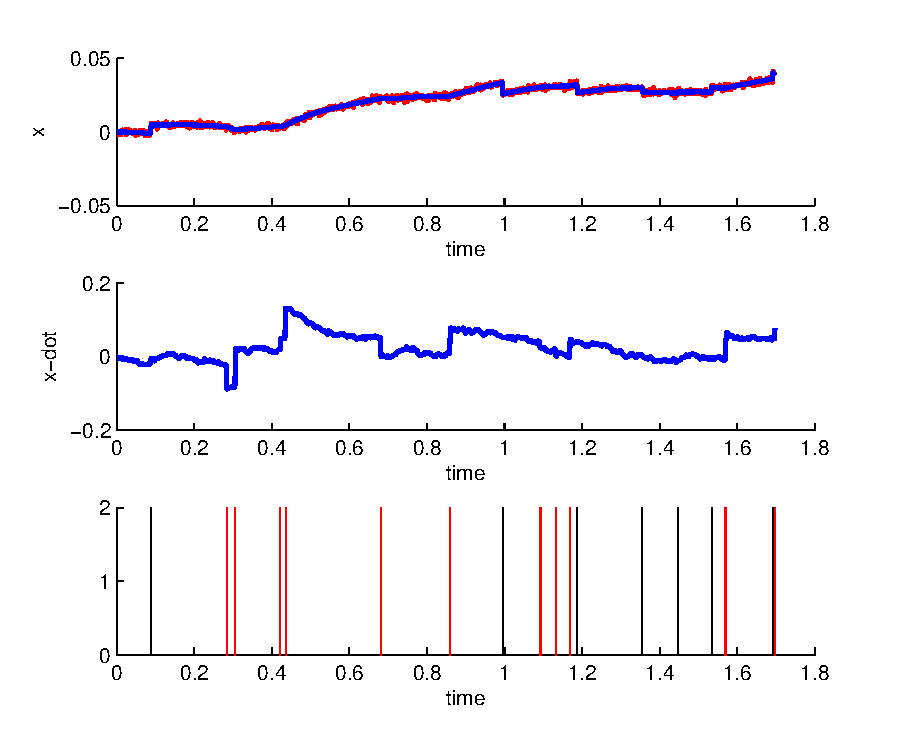
\includegraphics[width=0.95\columnwidth]{example_data.pdf}
\caption{An example simulated data set}
\label{fig:example_data}
\end{figure}

\begin{figure}[!t]
\centering
\subfloat[]{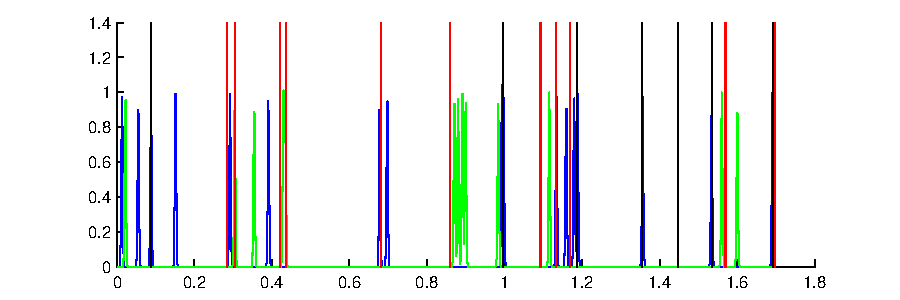
\includegraphics[width=0.95\columnwidth]{example_filter_kdest.pdf}} \\
\subfloat[]{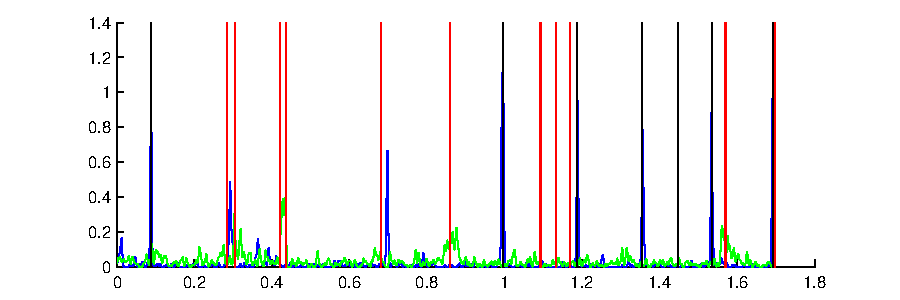
\includegraphics[width=0.95\columnwidth]{example_smoother_kdest.pdf}}
\caption{Filter (a) and smoother (b) kernel density estimates for value (blue) and trend (green) jump times. Correct times overlayed as vertical lines (black=value, red=trend).}
\label{fig:example_kdest}
\end{figure}

It is also possible to compare the algorithms via the accuracy of the state estimates they generate. Here we can compare three options: the filtering results, using the RBVRPF and a Kalman filter for the state estimates; the filter-smoother results, using the final RBVRPF approximation for the changepoint sequence and a Rauch-Tung-Striebel (RTS) smoother for the state estimates; and the smoothing results, using the RBVRPS followed by an RTS smoother. For the example run, these are shown in figure~\ref{fig:example_state}. Again, the improved particle diversity of the smoother is apparent.

\begin{figure}[!t]
\centering
\subfloat[]{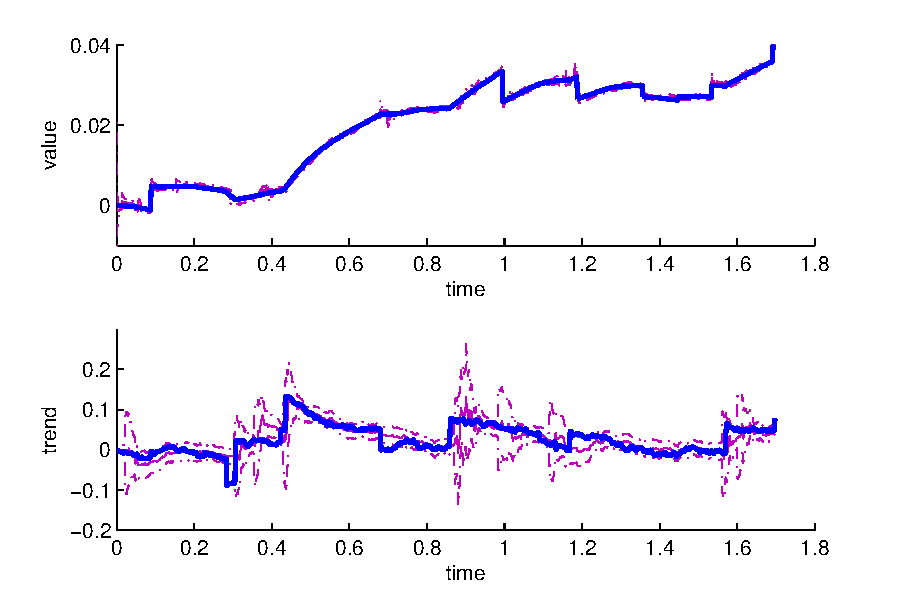
\includegraphics[width=0.95\columnwidth]{example_filter_state.pdf}} \\
\subfloat[]{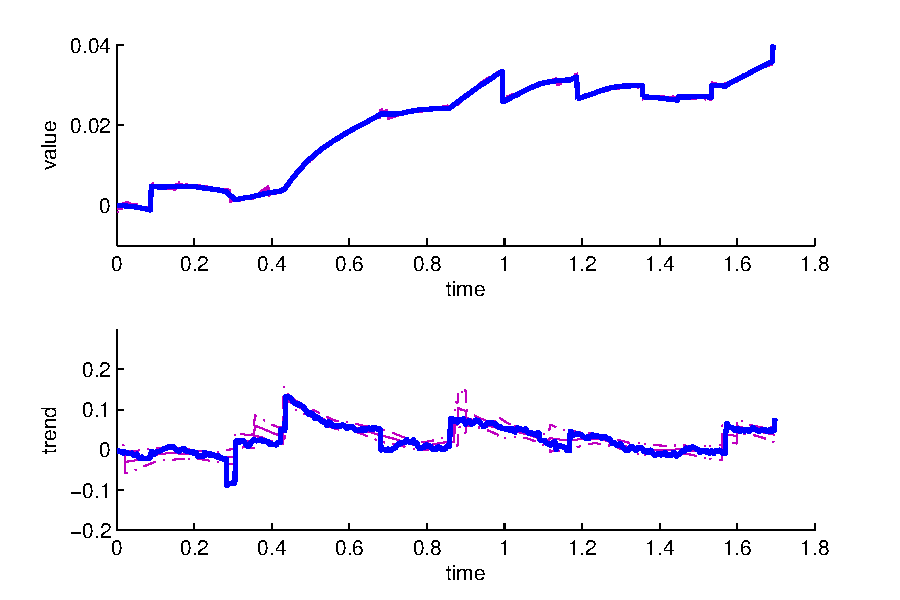
\includegraphics[width=0.95\columnwidth]{example_filtersmoother_state.pdf}} \\
\subfloat[]{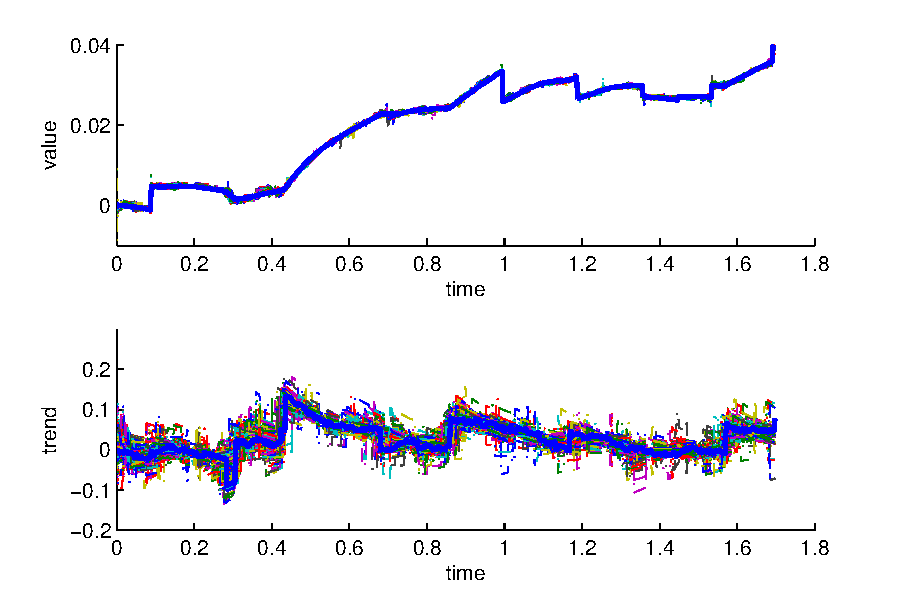
\includegraphics[width=0.95\columnwidth]{example_smoother_state.pdf}}
\caption{State estimates using RBVRPF + KF (a) final RBVRPF approximation + RTS smoother (b) and RBVRPS + RTS smoother. Solid lines show means of each particle. Dashed lines show mean $\pm$2 standard deviations.}
\label{fig:example_state}
\end{figure}

For quantitative comparison, the algorithms were tested on XX realisations from the model, and the following statistics were calculated for each:
\begin{itemize}
	\item The number of unique changepoint sequences. This is a measure of particle diversity of the approximation.
	\item The number of unique changepoint times. Another measure of particle diversity.
	\item The optimal sub-pattern assignment (OSPA) distance between the maximum a posteriori (MAP) changepoint sequence and the true sequence. The OSPA is a concept from multiple target tracking introduced in \cite{Schuhmacher2008} to measure the distance between sets of points of varying cardinality. It is thus well suited to measuring the error between changepoint sequences of varying length. For each approximation, the sequence from the MAP particle was used as a point estimate.
	\item The root-mean-square error (RMSE) of the MAP state estimate. The MAP state estimate is taken to be the Gaussian mean of the conditional state distribution, from the Kalman smoother or RTS, selected from the particle with the highest posterior probability.
	\item The root-mean-square error (RMSE) of the mean state estimate. The mean state estimate is the average of the Gaussian means from all the particles.
\end{itemize}

Note that the MAP particle may be found by calculating the posterior probability of each. The terms required for this calculation will already have been evaluated during the filtering procedure.

\begin{IEEEeqnarray}{rCl}
 p(\theta|y_{1:N}) & \propto & p(y_{1:N}|\theta) p(\theta) \nonumber \\
                         &         & S(\tau_K, T) \prod_{k=1}^K p(u_k) p(\tau_k|\tau_{k-1}) \prod_{n=1}^{N} p(y_n|\theta, y_{1:n-1})
\end{IEEEeqnarray}

The results are shown in tables~\ref{tab:cp_performance} and ~\ref{tab:state_performance}. The OSPA parameters are: exponent $p=1$, threshold $c=0.01$.

\begin{table}%
\begin{tabular}{|c|c|c|}
\hline
 & RBVRPF & RBVRPS \\
\hline
mean no. sequences   & 7.8      & 100       \\
mean no. jump times  & 47.8     & 1076.7    \\
MAP sequence OSPA    & $5.36 \times 10^{-3}$ & $4.98 \times 10^{-3}$  \\
\hline
\end{tabular}
\caption{Changepoint sequence estimation performance.}
\label{tab:cp_performance}
\end{table}

\begin{table}%
\begin{tabular}{|c|c|c|c|}
\hline
 & RBVRPF + KF & RBVRPF + RTS & RBVRPS + RTS \\
\hline
mean value estimate RMSE   & $5.31 \times 10^{-4}$ & $4.48 \times 10^{-4}$ & $4.16 \times 10^{-4}$ \\
mean trend estimate RMSE   & $2.56 \times 10^{-2}$ & $1.79 \times 10^{-2}$ & $1.49 \times 10^{-2}$ \\
MAP value estimate RMSE    & $5.98 \times 10^{-4}$ & $4.48 \times 10^{-4}$ & $4.49 \times 10^{-4}$ \\
MAP trend estimate RMSE    & $3.13 \times 10^{-2}$ & $1.79 \times 10^{-2}$ & $1.74 \times 10^{-2}$ \\
\hline
\end{tabular}
\caption{State estimation performance.}
\label{tab:state_performance}
\end{table}

The new RBVRPS algorithm outperforms the filter in all respects, both in terms of accuracy and particle diversity.

\begin{meta}
Another interesting question is how the posterior distribution over the number of changepoints is expected to behave. The prior is poisson distributed with mean $\alpha T$. The means of both the filter and smoother particle posterior are consistently greater than the true number (by about 50\%). Is this expected and why?
\end{meta}

Finally, we demonstrate the algorithms on a real financial data set, 1000 data points representing 1.7s of USD-GBP foreign exchange rate data from April 2008, using the same parameters as for the previous simulations. State estimates and jump time kernel density estimates are shown in figure~\ref{fig:fx_results}. In this example, there is no ground truth against which to judge the results. However, the smoother does a pleasing job of estimating jump times in the same areas that one would if analysing the data ``by eye''.

\begin{figure}[!t]
\centering
\subfloat[]{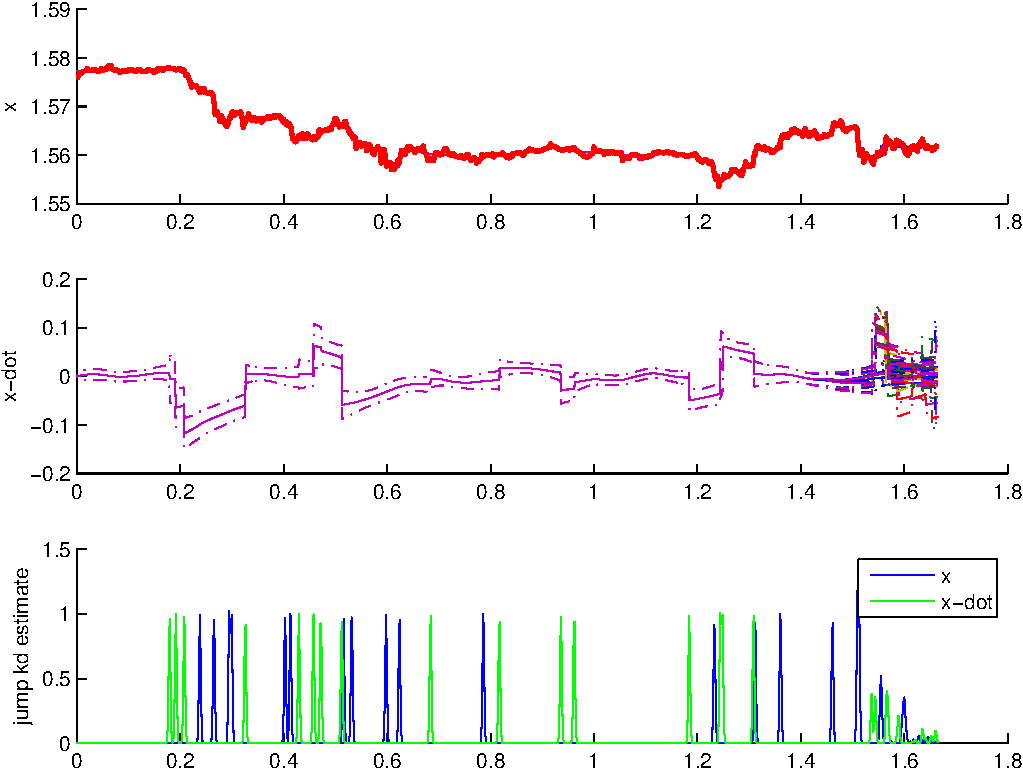
\includegraphics[width=0.95\columnwidth]{fx_filtersmoother-crop.pdf}} \\
\subfloat[]{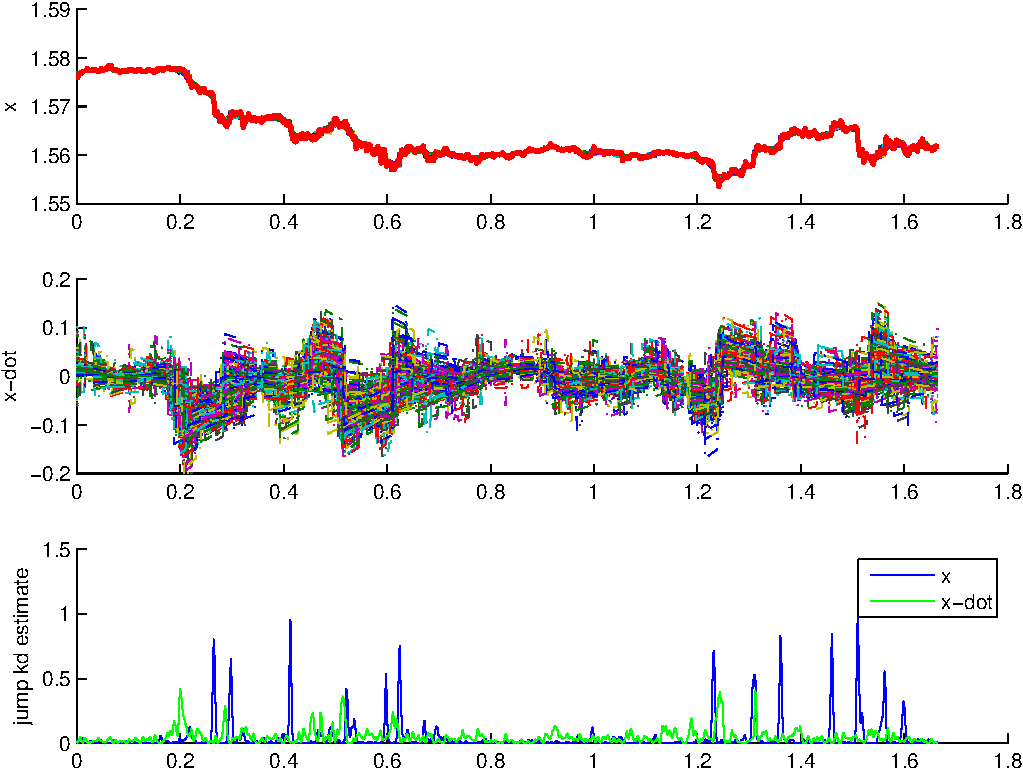
\includegraphics[width=0.95\columnwidth]{fx_smoother-crop.pdf}}
\caption{Filter (a) and smoother (b) state and kernel density estimates. State estimates show mean for each particle (solid) as well as mean $\pm$2 standard deviations (dashed). Kernel density estimates for value (blue) and trend (green) jump times.}
\label{fig:fx_results}
\end{figure}



\subsection{Tracking Application}

\begin{meta}
Add a tracking application here, in which the changepoints mark manoeuvre start points and there is a turn rate or acceleration parameter for each.
\end{meta}

% Template bits

% An example of a floating figure using the graphicx package.
% Note that \label must occur AFTER (or within) \caption.
% For figures, \caption should occur after the \includegraphics.
% Note that IEEEtran v1.7 and later has special internal code that
% is designed to preserve the operation of \label within \caption
% even when the captionsoff option is in effect. However, because
% of issues like this, it may be the safest practice to put all your
% \label just after \caption rather than within \caption{}.
%
% Reminder: the "draftcls" or "draftclsnofoot", not "draft", class
% option should be used if it is desired that the figures are to be
% displayed while in draft mode.
%
%\begin{figure}[!t]
%\centering
%\includegraphics[width=2.5in]{myfigure}
% where an .eps filename suffix will be assumed under latex,
% and a .pdf suffix will be assumed for pdflatex; or what has been declared
% via \DeclareGraphicsExtensions.
%\caption{Simulation Results}
%\label{fig_sim}
%\end{figure}

% Note that IEEE typically puts floats only at the top, even when this
% results in a large percentage of a column being occupied by floats.


% An example of a double column floating figure using two subfigures.
% (The subfig.sty package must be loaded for this to work.)
% The subfigure \label commands are set within each subfloat command, the
% \label for the overall figure must come after \caption.
% \hfil must be used as a separator to get equal spacing.
% The subfigure.sty package works much the same way, except \subfigure is
% used instead of \subfloat.
%
%\begin{figure*}[!t]
%\centerline{\subfloat[Case I]\includegraphics[width=2.5in]{subfigcase1}%
%\label{fig_first_case}}
%\hfil
%\subfloat[Case II]{\includegraphics[width=2.5in]{subfigcase2}%
%\label{fig_second_case}}}
%\caption{Simulation results}
%\label{fig_sim}
%\end{figure*}
%
% Note that often IEEE papers with subfigures do not employ subfigure
% captions (using the optional argument to \subfloat), but instead will
% reference/describe all of them (a), (b), etc., within the main caption.


% An example of a floating table. Note that, for IEEE style tables, the
% \caption command should come BEFORE the table. Table text will default to
% \footnotesize as IEEE normally uses this smaller font for tables.
% The \label must come after \caption as always.
%
%\begin{table}[!t]
%% increase table row spacing, adjust to taste
%\renewcommand{\arraystretch}{1.3}
% if using array.sty, it might be a good idea to tweak the value of
% \extrarowheight as needed to properly center the text within the cells
%\caption{An Example of a Table}
%\label{table_example}
%\centering
%% Some packages, such as MDW tools, offer better commands for making tables
%% than the plain LaTeX2e tabular which is used here.
%\begin{tabular}{|c||c|}
%\hline
%One & Two\\
%\hline
%Three & Four\\
%\hline
%\end{tabular}
%\end{table}


% Note that IEEE does not put floats in the very first column - or typically
% anywhere on the first page for that matter. Also, in-text middle ("here")
% positioning is not used. Most IEEE journals use top floats exclusively.
% Note that, LaTeX2e, unlike IEEE journals, places footnotes above bottom
% floats. This can be corrected via the \fnbelowfloat command of the
% stfloats package.



\section{Conclusion}
A new smoothing algorithm has been introduced for variable rate models which have linear-Gaussian system equations conditional on a set of unknown changepoint times. The algorithm employs the method of Rao-Blackwellisation, using a particle filter to estimate the nonlinear changepoint sequence, and Kalman filtering/smoothing methods to estimate the linear state components. The smoothing algorithm is shown to improve particle diversity and accuracy when compared to the filter.








\appendices
\section{Derivation of the Backwards Kalman Filter} \label{app:backward_filter}
Appendix one text goes here.

\section{Model Discretisation} \label{app:model_discretisation}
Appendix two text goes here.


% use section* for acknowledgement
\section*{Acknowledgment}


The authors would like to thank...


% Can use something like this to put references on a page
% by themselves when using endfloat and the captionsoff option.
\ifCLASSOPTIONcaptionsoff
  \newpage
\fi



% trigger a \newpage just before the given reference
% number - used to balance the columns on the last page
% adjust value as needed - may need to be readjusted if
% the document is modified later
%\IEEEtriggeratref{8}
% The "triggered" command can be changed if desired:
%\IEEEtriggercmd{\enlargethispage{-5in}}

% references section

% can use a bibliography generated by BibTeX as a .bbl file
% BibTeX documentation can be easily obtained at:
% http://www.ctan.org/tex-archive/biblio/bibtex/contrib/doc/
% The IEEEtran BibTeX style support page is at:
% http://www.michaelshell.org/tex/ieeetran/bibtex/
%\bibliographystyle{IEEEtran}
% argument is your BibTeX string definitions and bibliography database(s)
%\bibliography{IEEEabrv,../bib/paper}
%
% <OR> manually copy in the resultant .bbl file
% set second argument of \begin to the number of references
% (used to reserve space for the reference number labels box)
\bibliographystyle{IEEEtran}
\bibliography{D:/pb404/Dropbox/PhD/OTbib}

% biography section
%
% If you have an EPS/PDF photo (graphicx package needed) extra braces are
% needed around the contents of the optional argument to biography to prevent
% the LaTeX parser from getting confused when it sees the complicated
% \includegraphics command within an optional argument. (You could create
% your own custom macro containing the \includegraphics command to make things
% simpler here.)
%\begin{biography}[{\includegraphics[width=1in,height=1.25in,clip,keepaspectratio]{mshell}}]{Michael Shell}
% or if you just want to reserve a space for a photo:

\begin{IEEEbiographynophoto}{Pete Bunch}
Biography text here.
\end{IEEEbiographynophoto}

% if you will not have a photo at all:
\begin{IEEEbiographynophoto}{Simon Godsill}
Biography text here.
\end{IEEEbiographynophoto}

% insert where needed to balance the two columns on the last page with
% biographies
%\newpage

% You can push biographies down or up by placing
% a \vfill before or after them. The appropriate
% use of \vfill depends on what kind of text is
% on the last page and whether or not the columns
% are being equalised.

%\vfill

% Can be used to pull up biographies so that the bottom of the last one
% is flush with the other column.
%\enlargethispage{-5in}



% that's all folks
\end{document}


